\chapter{Quantum Electrodynamics}

The Lagrangian for quantum electrodynamics is
\begin{equation}
\begin{aligned}
	\mathcal{L}_{\mathrm{QED}}
	&= \bar\psi \left(i\gamma^\mu \partial_\mu - m\right)\psi - \frac{1}{4}F_{\mu\nu}F^{\mu\nu} -eA_\mu \bar\psi\gamma^\mu  \psi \\
	&= \mathcal{L}_{\mathrm{Dirac}}+\mathcal{L}_{\mathrm{Maxwell}}+\mathcal{L}_{\mathrm{int}},
\end{aligned}
\end{equation}
where
\begin{equation}
	F_{\mu\nu} = \partial_\mu A_\nu - \partial_\nu A_\nu = (dA)_{\mu\nu}.
\end{equation}
The Lagrangian is invariant under the gauge transformation:
\begin{equation}
\begin{aligned}
	\psi(x) &\rightarrow e^{-ie\alpha(x)}\psi(x), \\
	A^\mu(x) &\rightarrow A^\mu(x) + \partial^\mu \alpha(x).
\end{aligned}
\end{equation}
It is convenient to rewrite Lagrangian as
\begin{equation}
	\mathcal{L}_{\mathrm{QED}}
	= \bar\psi \left(i\cancel{D} - m\right)\psi - \frac{1}{4}F_{\mu\nu}F^{\mu\nu},
\end{equation}
where we have define the covariant derivative as:
\begin{equation}
	\cancel{D} = \gamma^\mu D_\mu 
	= \gamma^\mu [\partial_\mu + i e A_\mu(x)]
	= \cancel{\partial} + ie \cancel{A}.
\end{equation}


\section{Perturbative Renormalization}
As with the scalar field, 
\begin{equation}
	Z[\bar\eta,\eta,J] = \exp\left\{i\int d^dx \mathcal{L}_{\mathrm{int}}\left[\frac{\delta}{i\delta J},\frac{\delta}{i\delta \eta},\frac{i\delta}{\delta \bar\eta}\right]\right\} Z_0[\bar\eta,\eta,J].
\end{equation}
We use the dimensional regularization by default. 
Note that $\psi$ has the mass dimension $[\frac{d-1}{2}]$, $A^\mu$ had the mass dimension $[\frac{d}{2}-1]$, and $e$ has the mass dimension $[2-\frac{d}{2}]$.
When $d=4-\epsilon$, we make the replacement
\begin{equation}
	e \rightarrow e \tilde{\mu}^{\epsilon/2},
\end{equation}
so that to make the coupling constant $e$ dimensionless.

The renormalized Lagrangian is
\begin{equation}
\begin{aligned}
	\mathcal L 
		&= Z_{\psi} \bar\psi_R(i\gamma^\mu \partial_\mu)\psi_R 
		-Z_m m \bar\psi_R\psi_R 
		+ \frac{1}{4} Z_{A} F_{R,\mu\nu}F_R^{\mu\nu} - Z_e e_R A_R^\mu \bar\psi_R\gamma^\mu \psi_R \\
		&= \mathcal{L}_0 + \mathcal{L}_{\mathrm{int}} + \mathcal{L}_{\mathrm{ct}}.
\end{aligned}
\end{equation}
The we define the coefficients
\begin{equation}
	\delta_{\psi} = Z_\phi - 1,\ 
	\delta_{m} = Z_m - 1,\ 
	\delta_Z = Z_A - 1, \ 
	\delta_e = Z_e - 1.
\end{equation}
The counter term also contribute to the perturbative expansion like the interactions.
The counter terms for the fermion propagator come from the diagram expression:
\begin{equation}
\begin{aligned}
	iD_F^{\mathrm{(ct)}} 
	&= 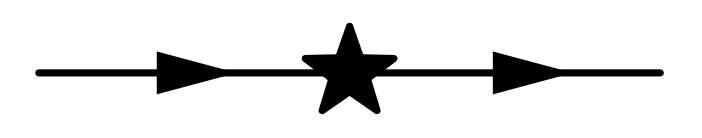
\includegraphics[align=c, width=0.25\linewidth]{pics/QED-ct-1.png} \\
	&\sim \frac{\delta^2}{\delta\bar\eta \delta\eta}
	i(\delta_{\psi}\gamma^\mu_{\alpha\beta}k_\mu-\delta_m \mathbb{I}_{\alpha\beta})\frac{\delta^2}{\delta\eta_{\alpha} \delta\bar\eta_{\beta}}
	\frac{1}{2!}\left(-i \bar\eta_{\alpha} D_F^{\alpha\beta} \eta_{\beta} \right)^2.
\end{aligned}
\end{equation}
The contribution to the electron self energy is
\begin{equation}
	i\Sigma(p) = \delta_{\psi}\cancel{p}-\delta_m m_R.
\end{equation}
Similarly, the counter term contribution to the photon self energy is
\begin{equation}
\begin{aligned}
	i \Sigma^{\mu\nu}(k) 
	&= 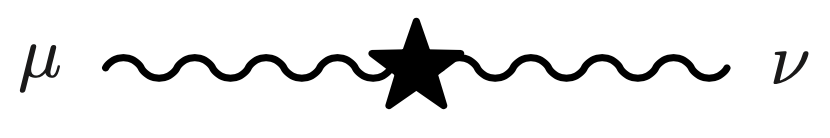
\includegraphics[align=c,width=0.25\linewidth]{pics/QED-ct-2.png} \\
	&= \delta_A [-p^2 g^{\mu\nu} + (1-\xi)p^\mu p^\nu].
\end{aligned}
\end{equation}
And the counter term contribution to the QED vertex is
\begin{equation}
	i\Gamma^{\mu}_{\alpha\beta} 
	= 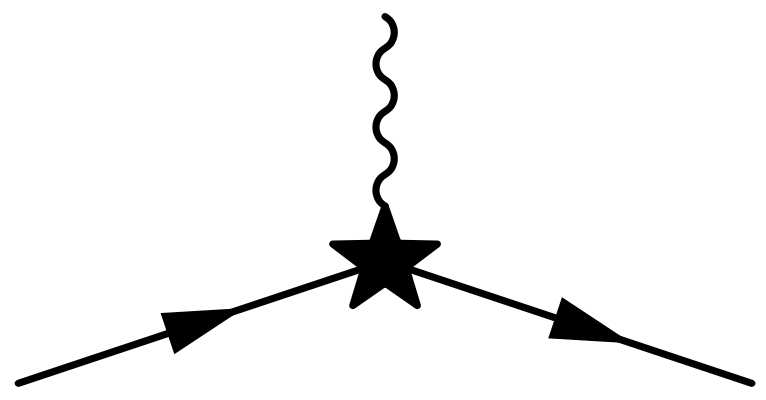
\includegraphics[align=c, width=0.2\linewidth]{pics/QED-ct-3.png} 
	= \delta_e \gamma^{\mu}_{\alpha\beta}.
\end{equation}



\subsection{One-loop Correction to Electron Propagator}

Consider the one-loop correction to the particle propagator:
\begin{equation}
	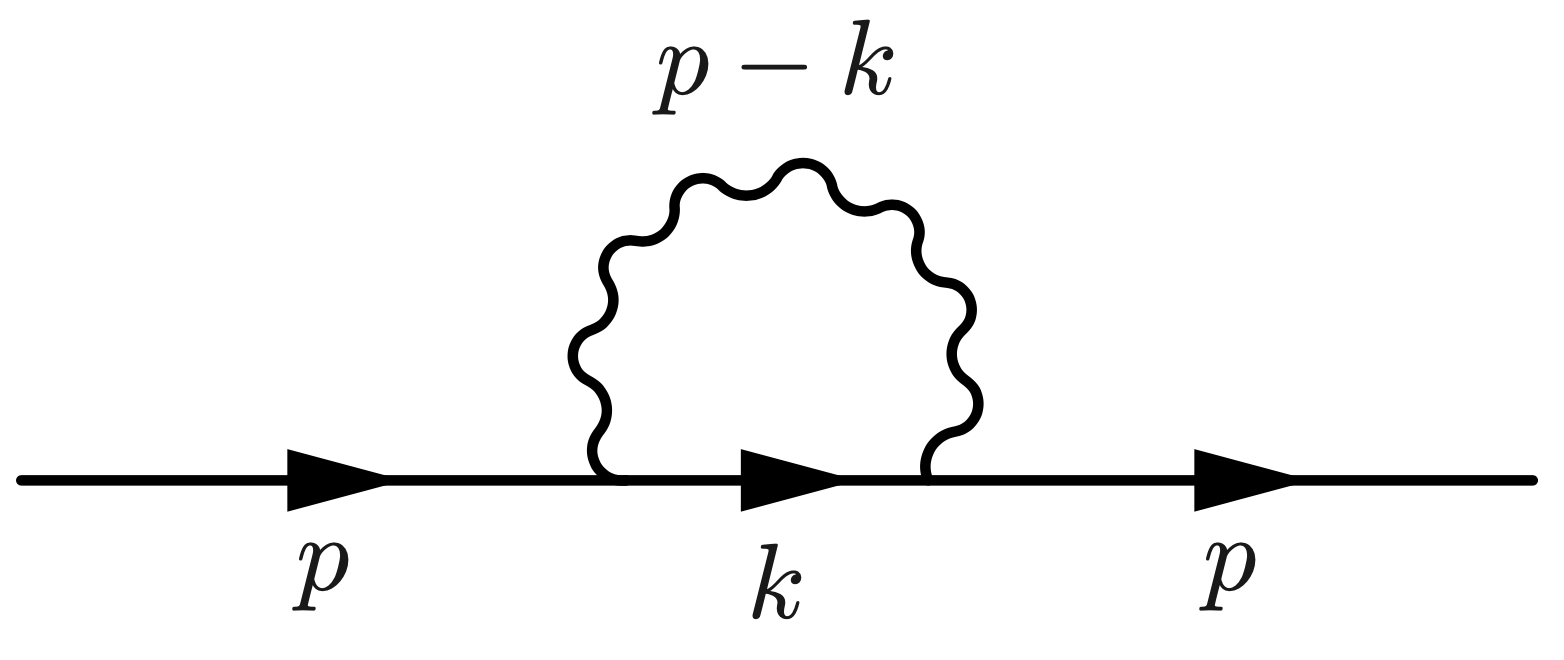
\includegraphics[width=0.2\linewidth,align=c]{pics/QED-1.png} \simeq (-ie)^2\wick{
		\c1{A}_\mu \bar\psi_\alpha \gamma^\mu_{\alpha\gamma} \c2{\psi}_\gamma
		\c1{A}_\nu \c2{\bar\psi}_\tau \gamma^\nu_{\tau\beta} \psi_\beta}
	\equiv i\bar\psi_\alpha \Sigma^{\alpha\beta}(p) \psi_\beta.
\end{equation}
The self energy is
\begin{equation}
\begin{aligned}
	i\Sigma_{\alpha\beta}(p)
	&= e^2\int\frac{d^4 k}{(2\pi)^4} \Pi_{\mu\nu}(p-k) \left[\gamma^\mu D_F(k) \gamma^\nu\right]_{\alpha\beta} \\
	&= -e^2\int\frac{d^d k}{(2\pi)^d}\frac{\gamma^\mu(\cancel{k}+m)\gamma_\mu}{(p-k)^2(k^2-m^2)}.
\end{aligned}
\end{equation}
The seconded equality comes from the contraction:
\begin{equation}
	(-ie)^2\wick{
		\c1{A}_\mu \bar\psi_\alpha \gamma^\mu_{\alpha\gamma} \c2{\psi}_\gamma
		\c1{A}_\nu \c2{\bar\psi}_\tau \gamma^\nu_{\tau\beta} \psi_\beta}
\end{equation}
The nominator can be simplified using the Dirac matrix identities:
\begin{equation}
	\gamma^\mu \gamma_\mu = 4, \
	\gamma^\mu \gamma^\nu \gamma_\mu = -2 \gamma^\nu
	\quad \Rightarrow \quad
	\gamma^\mu(\cancel{k}+m)\gamma_\mu = 4 m-2\cancel{k}.
\end{equation}
The denominator can be simplify using the Feynman parameter:
\begin{equation*}
	\frac{1}{(p-k)^2(k^2-m^2)} = \int_0^1 \frac{dx}{\left[(k-b)^2-D\right]^2}
\end{equation*}
where $b$ and $D$ can be calculated by
\begin{lstlisting}[style=mathematicaFrameTB]
A1=(k-p)^2;
A2=k^2-m^2;
{c,b,a}=CoefficientList[x*A1+(1-x)*A2,{k}];
-b/2
-c+b^2/(4*a)//Simplify
\end{lstlisting}
The result is $b = p x$ and $D = (1-x)(m^2-p^2 x)$.
Shift $k \rightarrow k + px$, the self energy becomes (including a $\tilde \mu$ mass scale):
\begin{equation}
\begin{aligned}
	i\Sigma(p)
	&= 2e^2\tilde{\mu}^{\epsilon} 
		\int_0^1 (x\cancel{p}-2m)dx 
		\int \frac{d^d k}{(2\pi)^d} 
		\frac{1}{(k^2-D)^2} \\
	&= i\frac{2e^2 \tilde{\mu}^{\epsilon}\Omega_d}{(2\pi)^d}
		\int_0^1 (x\cancel{p}-2m)dx
		\int \frac{k^{d-1} dk}{(k^2+D)^2}.
\end{aligned}
\end{equation}
The regularization procedure is
\begin{lstlisting}[style=mathematicaFrameTB]
omg=(2*Pi^(d/2))/(Gamma[d/2]);
cof=2*e^2*\[Mu]^(4-d)*omg/(2*Pi)^d;
int=cof*Integrate[q^(d-1)/(q^2+D)^2,{q,0,Infinity}][[1]];
map={e->Sqrt[4*Pi*\[Alpha]],EulerGamma->Subscript[\[Gamma],E]};
ans=Series[int/.{d->4-\[Epsilon]},{\[Epsilon],0,0}];
ans/.map//Simplify
\end{lstlisting}
The result is ($\mu^2 = 4\pi \tilde\mu^2 e^{-\gamma_E}$)
\begin{equation}
	\Sigma(p) = \frac{e_R^2}{8\pi^2}\int_0^1 dx(x\cancel{p}-2m_R)\left[\frac{2}{\epsilon}+\ln\left(\frac{\mu^2}{D}\right)\right].
\end{equation}
The infinity comes from
\begin{equation}
	\frac{e_R^2}{4\pi^2\epsilon}\int_0^1 dx(x\cancel{p}-2m_R)
	= \frac{e_R^2}{8\pi^2\epsilon}\cancel{p} - \frac{e_R^2}{2\pi^2\epsilon}m_R.
\end{equation}
Using the $\overline{\mathrm{MS}}$ subtraction scheme, we choose
\begin{equation}
	\delta_{\psi} = -\frac{e_R^2}{8\pi^2\epsilon},\ 
	\delta_m = -\frac{e_R^2}{2\pi^2\epsilon},
\end{equation}
and the self energy is
\begin{equation}
\begin{aligned}
	\Sigma(p) 
	&= \frac{e_R^2}{8\pi^2}\int_0^1 dx(x\cancel{p}-2m_R)\ln\left[\frac{\mu^2}{(1-x)(m_R^2-p^2 x)}\right] \\
	&= \frac{e_R^2}{8\pi^2}(\cancel{p}-4m_R)\ln\left(\frac{\mu}{m_R}\right)-\int_0^1 dx \ln\left[(1-x)\left(1-\frac{p^2x}{m_R^2}\right)\right].
\end{aligned}
\end{equation}



\subsection{One-loop Correction to Photon Propagator}
Consider the one-loop correction to the photon propagator:
\begin{equation}
	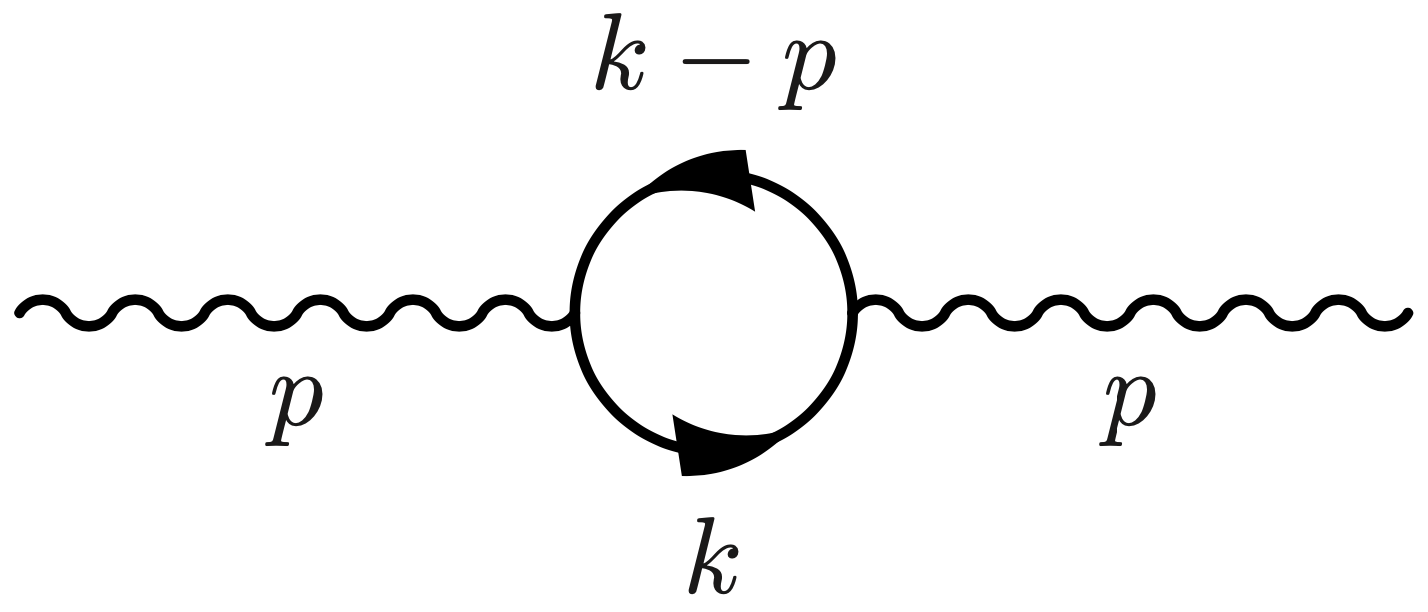
\includegraphics[align=c,width=0.15\linewidth]{pics/QED-2.png} 
	\simeq (-ie)^2\wick{
		A_\mu \c2{\bar\psi}_\alpha \gamma^\mu_{\alpha\beta} \c1{\psi}_\beta 
		A_\nu \c1{\bar\psi}_\gamma \gamma^\nu_{\gamma\tau} \c2{\psi}_\tau
	} \equiv iA_\mu \Pi^{\mu\nu}(p) A_\nu.
\end{equation}
The self energy is:
\begin{equation}
\begin{aligned}
	i\Sigma^{\mu\nu}(p) 
	&= -e^2 \int\frac{d^4 k}{(2\pi)^4} \mathrm{Tr}\left[\gamma^\mu D_F(k-p) \gamma^\nu D_F(k) \right] \\
	&= -e^2 \int\frac{d^4 k}{(2\pi)^4} 
	\frac{\mathrm{Tr}\left[\gamma^\mu (\cancel k- \cancel p +m) \gamma^\nu (\cancel k +m) \right]}{(k^2-m^2)[(p-k)^2-m^2]}.
\end{aligned}
\end{equation}
The Dirac trace and Feynman parameter is calculated by the following code:

\begin{lstlisting}[style=mathematicaFrameTB]
(*Dirac trace using FeynCalc`*)
DiracTrace[GA[\[Mu]].(GS[k-p]+m).GA[\[Nu]].(GS[k]+m)]//DiracSimplify

(*Feynman paramater*)
A1=k^2-m^2;
A2=(k-p)^2-m^2;
{c,b,a}=CoefficientList[x*A1+(1-x)*A2,{k}];
-b/2
-c+b^2/(4*a)//Simplify
\end{lstlisting}

The nominator is
\begin{equation}
	4 \left[g^{\mu\nu} \left(k\cdot p-{k}^2+m^2\right)+ 2k^\mu k^\nu - k^\mu p^\nu - p^\mu k^\nu \right].
\end{equation}
The denominator is:
\begin{equation}
	\frac{1}{(k^2-m^2)[(p-k)^2-m^2]}
	= \frac{1}{\left\{[k-p(1-x)]^2-[m^2+p^2 x(x-1)]\right\}^2}.
\end{equation}
Let $D=m^2-p^2 x(1-x)$, shift $k \rightarrow k + p(1-x)$, and drop all $p^\mu$ linear term,\footnote{The Ward identity requires that the $p^\mu$ term in the propagator do not contribute to any scattering process.} the result is
\begin{equation}
	i\Sigma^{\mu \nu}= -4 e^{2}\tilde{\mu}^{\epsilon} \int_0^1 dx
		\int \frac{d^{d} k}{(2 \pi)^{d}}  \frac{2 k^{\mu} k^{\nu}-g^{\mu \nu}\left[k^{2}-x(1-x) p^{2}-m^{2}\right]}{\left[k^{2}-D\right]^{2}}.
\end{equation}
The self-energy $i\Sigma^\mu \propto g^{\mu\nu}$, we can make the substitution
\begin{equation*}
	k^\mu k^\nu \rightarrow \frac{1}{d} k^2 g^{\mu\nu}.
\end{equation*}
We then need to consider the integral
\begin{equation*}
\begin{aligned}
	iI(x) &= 4e^2\tilde{\mu}^{\epsilon} \int\frac{d^d k}{(2 \pi)^{d}}  
		\frac{(1-\frac{2}{d})k^{2}-x(1-x) p^{2}-m^{2}}{\left[k^{2}-D\right]^{2}}, \\
	I(x) &= -\frac{4e^2\tilde{\mu}^{\epsilon} \Omega_d }{(2\pi)^d}
		\int k^{d-1} dk \frac{(1-\frac{2}{d})k^{2}+x(1-x) p^{2}+m^{2}}{\left[k^{2}+D\right]^{2}}.
\end{aligned}
\end{equation*}
The regulation is carried out by the following code:
\begin{lstlisting}[style=mathematicaFrameTB]
omg=(2*Pi^(d/2))/(Gamma[d/2]);
cof=-4*e^2*\[Mu]^(4-d)*omg/(2*Pi)^d;
den=q^(d-1)*((1-2/d)q^2+x*(1-x)p^2+m^2);
int=cof*Integrate[den/(q^2+D)^2,{q,0,Infinity}][[1]];
map={EulerGamma->Subscript[\[Gamma],E],D->m^2-p^2*x*(1-x)};
ans=Series[int/.{d->4-\[Epsilon]},{\[Epsilon], 0, 0}];
ans/.map//Simplify
\end{lstlisting}
The result is
\begin{equation}
	\Sigma^{\mu\nu}(p) 
	= -\frac{e_R^2 p^2 g^{\mu\nu}}{2\pi^2} \int_0^1 dx\ x(1-x)
	\left[\frac{2}{\epsilon}+\ln\left(\frac{\mu^2}{m_R^2-p^2 x(1-x)}\right)\right]
\end{equation}
The divergent part is
\begin{equation*}
	-\frac{e_R^2 p^2 g^{\mu\nu}}{\pi^2 \epsilon} \int_0^1 dx\ x(1-x)
	= -\frac{e_R^2 p^2 g^{\mu\nu}}{6\pi^2 \epsilon}.
\end{equation*}
The counter term coefficient is
\begin{equation}
	\delta_A = -\frac{e_R^2}{6\pi^2 \epsilon}.
\end{equation}
The photon self-energy is then
\begin{equation}
\begin{aligned}
	\Sigma^{\mu\nu}(p) 
	&= -\frac{e_R^2 p^2 g^{\mu\nu}}{2\pi^2} \int_0^1 dx\ x(1-x)
	\ln\left[\frac{\mu^2}{m_R^2-p^2 x(1-x)}\right] \\
	&= -\frac{e_R^2 p^2 g^{\mu\nu}}{12\pi^2} \ln\left(\frac{\mu}{m}\right)
	 + \frac{e_R^2 p^2 g^{\mu\nu}}{2\pi^2}\int_0^{1} dx\ x(1-x) \ln\left[1-\frac{p^2}{m_R^2}x(1-x)\right].
\end{aligned}
\end{equation}






\subsection{One-loop Correction to Vertex}
Consider the one-loop correction to interaction:
\begin{equation}
\begin{aligned}
	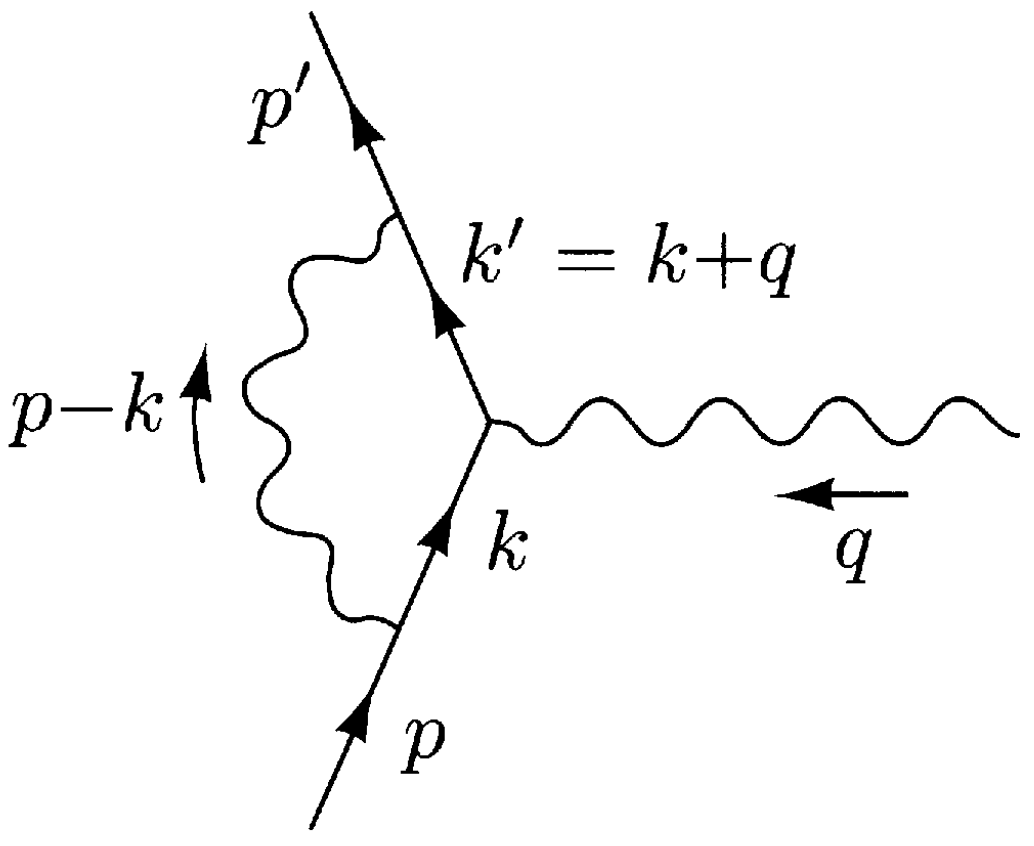
\includegraphics[align=c,width=0.23\linewidth]{pics/QED-3.png}
	& \simeq (-ie)^3\wick{
		\c1{A}_\nu \bar\psi_\alpha \gamma^\nu_{\alpha\beta} \c2{\psi}_\beta 
		A_\mu \c2{\bar\psi}_\lambda \gamma^\mu_{\lambda\tau} \c3{\psi}_\tau
		\c1{A}_\xi \c3{\bar\psi}_\rho \gamma^\nu_{\rho\sigma} \psi_\sigma
	} \\ &\equiv -ie A_\mu \Gamma^\mu_{\alpha\beta}(q,p,p') \bar\psi_\alpha \psi_\beta.
\end{aligned}
\end{equation}
The vertex function is:
\begin{equation}
\begin{aligned}
	i\Gamma^\mu_{\alpha\beta}(q,p,p')
	&= -e^2 \int\frac{d^4 k}{(2\pi)^4} 
	\Pi_{\nu\lambda}(p-k) 
	[\gamma^\nu D_F(k') \gamma^\mu D_F(k) \gamma^\lambda]_{\alpha\beta} \\
	&= e^2 \int\frac{d^4 k}{(2\pi)^4} 
	\frac{[\gamma^\nu(\cancel{k}'+m)\gamma^\mu (\cancel{k}+m)\gamma_\nu]_{\alpha\beta}}{(k^2-m^2)(k'^2-m^2)(p-k)^2}
\end{aligned}
	\label{eq:QED-loop-vertex}
\end{equation}
Using the following code
\begin{lstlisting}[style=mathematicaFrameTB]
(*numerator*)
den=Contract[GA[\[Nu]].(GS[kp]+m).GA[\[Mu]].(GS[k]+m).GA[\[Nu]]];
DiracSimplify[den]

(*Feynman parameter*)
A1=k^2-m^2;
A2=(k+q)^2-m^2;
A3=(p-k)^2;
{c,b,a}=CoefficientList[x*A1+y*A2+z*A3,{k}];
-b/2//Simplify
-c+b^2/4//Simplify
\end{lstlisting}
The numerator is
\begin{equation*}
	-2\cancel{k}\gamma^\mu\cancel{k}'-2m^2\gamma^\mu + 4m(k + k')^\mu.
\end{equation*}
The denominator is
\begin{equation*}
	\int \frac{dF_3}{[(k+yq-zp)^2-D]^3},
\end{equation*}
where 
\begin{equation*}
\begin{aligned}
	D &= (x+y)m^2 - z(1-z)p^2- y(1-y)q^2-2yzpq \\
	&=(x+y)m^2 - xy q^2- yz p'^2 - xz p^2.
\end{aligned}
\end{equation*}
Shift $k^\mu \rightarrow k^\mu + z q_1^\mu - y p^\mu$, throw away all terms with linear $k^\mu$, and replace $k^\mu k^\nu$ with $\frac{1}{d}k^2 g^{\mu\nu}$, the result is
\begin{equation*}
	\frac{4}{d}k^2\gamma^\mu  -2(-y \cancel{q}+z \cancel{p}) \gamma^{\mu}[(1-y) \cancel q+z \cancel p] +4 m^{2} \gamma^{\mu}-2 m\left[(1-2 y) q^{\mu}+2 z p^{\mu}\right].
\end{equation*}
Note that only the quadratic term is divergent. 
\begin{equation*}
	\Gamma^\mu(p,q_1,q_2) = -i\frac{4e^2\tilde{\mu}^{\epsilon} \gamma^\mu}{d}  \int dF_3 \int \frac{d^dk}{(2\pi)^d} \frac{k^2}{(k^2-D)^3} + \delta\Gamma^\mu(p,q_1,q_2).
\end{equation*}
where $\delta \Gamma^\mu$ stores all the finite part
\begin{equation*}
\begin{aligned}
	& \delta\Gamma^\mu(p,q_1,q_2) \\
	=& \int \frac{e^2 k^3 dk dF_3}{(2\pi)^2(k^2+D)^3} \left\{(-y \cancel{q}+z \cancel{p}) \gamma^{\mu}[(1-y) \cancel q+z \cancel p] -2 m^{2} \gamma^{\mu}+ m\left[(1-2 y) q^{\mu}+2 z p^{\mu}\right]\right\}.
\end{aligned}
\end{equation*}
The divergent part is
\begin{equation*}
	\frac{4 e^2\tilde{\mu}^{\epsilon} \Omega_d \gamma^\mu}{d(2\pi)^d}\int dF_3 \int \frac{k^{d+1}dk}{(k^2+D)^3}
	= \frac{e_R^2}{16\pi^2} \gamma^\mu \int dF_3 \left[\frac{2}{\epsilon}+\ln\left(\frac{\mu^2}{D}\right)\right].
\end{equation*}
Using the $\overline{\mathrm{MS}}$ scheme, the coefficient of the counter term is
\begin{equation}
	\delta_e = -\frac{e_R^2}{8\pi^2\epsilon}.
\end{equation}


\subsection{Renormalization Group}
In summery, the renormalization factors are
\begin{equation}
\begin{aligned}
	Z_\psi &= 1 -\frac{e_R^2}{8\pi^2\epsilon} + O(e_R^3), \\
	Z_A &= 1 - \frac{e_R^2}{6\pi^2 \epsilon} + O(e_R^3), \\
	Z_m &= 1 - \frac{e_R^2}{2\pi^2\epsilon} + O(e_R^3), \\
	Z_e &= 1 - \frac{e_R^2}{8\pi^2\epsilon} + O(e_R^3),
\end{aligned}
\end{equation}
which means
\begin{equation}
\begin{aligned}
	\frac{d\ln Z_\phi}{d e_R} &= -\frac{e_R}{4\pi^2 \epsilon} + O(e_R^2), \\
	\frac{d\ln Z_A}{d e_R} &= -\frac{e_R}{3\pi^2 \epsilon} + O(e_R^2), \\
	\frac{d\ln Z_m}{d e_R} &= -\frac{e_R}{\pi^2 \epsilon} + O(e_R^2), \\
	\frac{d\ln Z_e}{d e_R} &= -\frac{e_R}{4\pi^2 \epsilon} + O(e_R^2).
\end{aligned}
\end{equation}
The bare parameters are
\begin{equation}
\begin{aligned}
	\psi_0 &= Z_\psi^{1/2}\psi_R, \\
	A_0 &= Z_A^{1/2} A_R, \\
	m_0 &= Z_m Z_\psi^{-1} m_R, \\
	e_0 &= Z_e Z_\psi^{-1} Z_A^{-1/2} e_R \tilde{\mu}^{\epsilon/2}. 
\end{aligned}
\end{equation}
The RG equation for $e_0$ is
\begin{equation}
	\frac{d\ln e_0}{d\ln \mu}
	= \left(\frac{\ln Z_e}{d e_R} - \frac{\ln Z_\psi}{d e_R} - \frac{1}{2} \frac{\ln Z_A}{d e_R} + \frac{1}{e_R} \right)\frac{de_R}{d\ln \mu} + \frac{\epsilon}{2} = 0.
\end{equation}
The beta function is
\begin{equation}
	\beta(e_R) = \frac{de_R}{d\ln \mu} = -\frac{\epsilon}{2}e_R + \frac{e_R^3}{12\pi^2} + O(e_R^4).
\end{equation}
The RG equation for $m_0$ is
\begin{equation}
	\frac{d\ln m_0}{d\ln \mu}
	= \left(\frac{\ln Z_m}{d e_R} - \frac{\ln Z_\psi}{d e_R}\right)\frac{de_R}{d\ln \mu} + + \frac{1}{m_R}\frac{d m_R}{d\ln\mu} = 0.
\end{equation}
The anomalous dimension of mass is
\begin{equation}
	\gamma_m = \frac{d \ln m_R}{d\ln\mu} = -\frac{3e_R^2}{8\pi^2} + O(e_R^3).
\end{equation}



